\begin{frame}[fragile]{Issues in Word Representation}

  \begin{itemize}
    \item Words are often represented as one-hot encoding in computer.
    \item For example, we can set hotel and motel to two different
          representative as one-hot encoding:
          \begin{center}
            $$
              {v_{motel}}=\begin{pmatrix} 1 \\ 0 \\ 0 \\ \vdots \\ 0 \end{pmatrix},\;
              {v_{hotel}}=\begin{pmatrix} 0 \\ 1 \\ 0 \\ \vdots \\ 0 \end{pmatrix},\;
            $$
          \end{center}
  \end{itemize}

\end{frame}

\begin{frame}[fragile]{Issues in Word Representation}

  \begin{itemize}
    \item However, there are several issues when words are represented as one-hot encoding:
          \begin{enumerate}
            \item We cannot gain information of relation between words.
                  \begin{itemize}
                    \item We have no idea how motel and hotel are relate to each other while those two vectors are \textcolor{red}{orthogonal}! i.e. $ \langle v_{motel} , \; v_{hotel} \rangle = 0$
                  \end{itemize}
            \item The vector would be very sparse if there exists large amount of unique words.
          \end{enumerate}
    \item That's why we introduce word embedding approach to tackle these problems. \cite{word2vec}
  \end{itemize}

\end{frame}

\begin{frame}[fragile]{Word Embedding}

  \begin{center}
    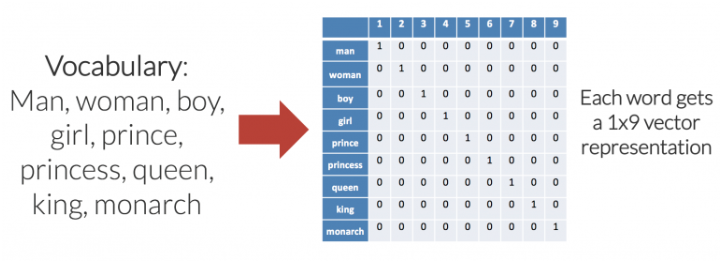
\includegraphics[scale=0.3]{../images/img_2.png} \\
    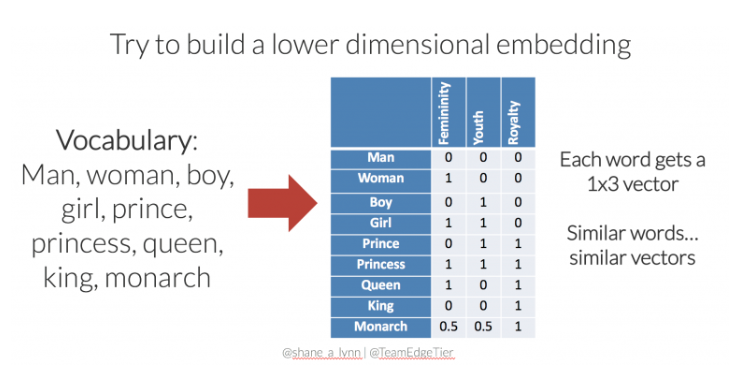
\includegraphics[scale=0.3]{../images/img_3.png} \\
    \href{https://www.shanelynn.ie/get-busy-with-word-embeddings-introduction/}{[Image Source]}
  \end{center}

\end{frame}

\begin{frame}[fragile]{Word2Vec}

  \begin{center}
    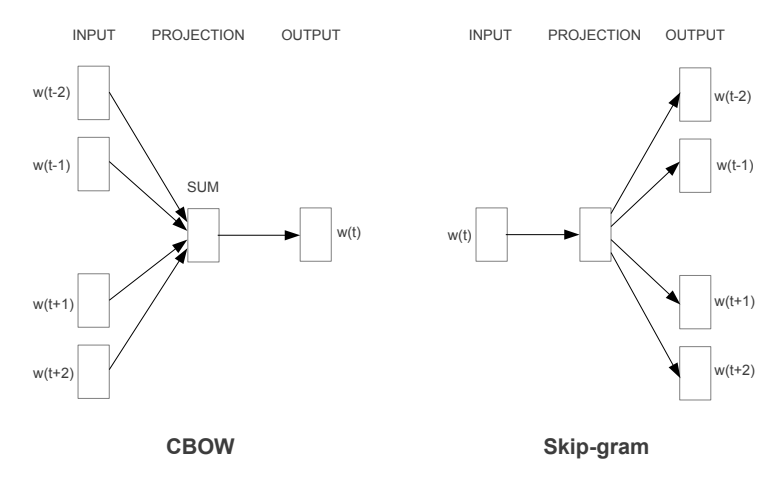
\includegraphics[scale=0.3]{../images/img_4.png} \\
    \href{https://arxiv.org/pdf/1301.3781.pdf}{[Image Source]}
  \end{center}

\end{frame}

\begin{frame}[fragile]{CBOW}

  \begin{center}
    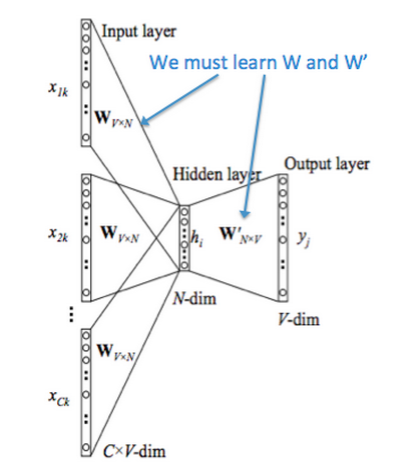
\includegraphics[scale=0.3]{../images/img_5.png} \\  \href{https://web.stanford.edu/class/archive/cs/cs224n/cs224n.1214/readings/cs224n-2019-notes01-wordvecs1.pdf}{[Image Source]}
  \end{center}

  \begin{itemize}
    \item Use probability $P(y_{i} | x_{1k}, x_{2k}, ... , x_{Ck})$ to learn the weight matrix $W$!
    \item $W$ is used to be the pre-trained model when we transform the words into embedding vectors in the unseen documents.
  \end{itemize}

\end{frame}